\section{Image Reconstruction for MeerKAT} \label{intro}
In the real world, measurements are corrupted by noise. Noise is introduced by the measurement instrument itself, but additional interference sources may be present. For example in Audio Recording, the microphone measures a noisy signal from the real world tone, and a passing car introduces additional interference. In a controlled environment like a recording studio, sound proofing handles the interference and only the noisy measurements have to be dealt with. Controlled environments are not always possible, that's why in Signal Processing the fields of de-noising and reconstruction exists. With those, we want to reconstruct the truly observed signal without the noise or external interference.

Image de-noising and reconstruction problems appear in different fields. In Astronomy, Radio Interferometers pose a challenging image reconstruction problem. The Interferometer measures a noisy image of the sky, corrupted by various sources like the ionosphere, passing satellites and the Interferometer itself. In the past, reconstruction algorithms used simple approximations to correct the image. For new interferometers like MeerKAT the approximations of the past do not hold. Furthermore, the larger MeerKAT instrument poses the reconstruction problem on a new data volume. 

Reconstruction algorithms for MeerKAT should handle the more complex effects of ionosphere and the like, while scaling even more on larger problem instances. Reconstruction algorithms using the theory of compressed sensing\cite{candes2006robust}\cite{donoho2006compressed} showed higher reconstruction accuracy than state of the art algorithms. However, they currently do require more computing hardware. This project searches for a way to make CS Algorithm scale on MeerKAT data size.

SASIR\cite{starck2015starlet} or more recently reconstructions using SARA \cite{dabbech2018cygnus} \cite{birdi2018sparse}

\subsection{The basic Measurement Equation of a radio interferometer}
Real world radio interferometers have complicated measurement equations. They become even more complicated for large interferometers like MeerKAT. These problems get addressed in section \ref{meerkat}. This section looks at the basic measurement equation of a radio interferometer \eqref{intro:measurement} and discusses the two fundamental challenges for image reconstruction. 

\begin{equation}\label{intro:measurement}
V(u, v) = \int\int I(x, y) e^{2 \pi i (ux+vy)} \: dx \: dy
\end{equation}

An interferometer measures Fourier Components $V$ (called Visibilities in Radio Astronomy) from the sky image $I$ at position $x$ and $y$. The term $e^{2 \pi i (ux+vy)}$ represents the two dimensional Fourier Transform. The task is to reconstruct the observed image $I$ from the measured Visibilities $V$. In theory this task is trivial: Since the inverse Fourier Transform exists, we can reconstruct the image $I$ by calculating the inverse Fourier Transform of $V$. However, two properties of the Visibilities make this task challenging in practice:

\begin{enumerate}
	\item Non-uniform sampling pattern in Visibility space
	\item Incomplete Visibility coverage. 
\end{enumerate} 

\textit{Property 1:} We want to reconstruct an image with uniformly spaced pixels. The instrument defines the sampling pattern in Visibility space and does not correspond to the exact pixels of the reconstructed image. This property keeps us from using the Fast Fourier Transform. The naive inverse Fourier Transform can still be calculated, but it has a quadratic runtime and does not scale to the data volume of interferometers. Current reconstruction algorithms use the non-uniform Fast Fourier Transform (nuFFT). The nuFFT approximates the non-uniform Fourier Transform. 

\textit{Property 2:} Interferometers sample only a limited set of Visibilities. It does not have the whole information for reconstruction. This has the effect that the instrument introduces fake structures into the image. With only knowing the incomplete set of Visibilities, a reconstruction algorithm has to decide which image structures were truly measured, and which are due to the instrument. This forms an ill-posed inverse problem. There are many images that fit the measurements, and a small change in the Visibilities can lead to a very different reconstruction.

MeerKAT uses the WSCLEAN\cite{wsclean} for its image reconstruction. WSCLEAN is the state of the art reconstruction and is based on the CLEAN algorithm\cite{rich2008multi}\cite{rau2011multi}. After the inverse Fourier Transform, the CLEAN algorithms try to remove the instrumental effects from the image with a deconvolution: The incomplete Visibility coverage convolves the image with a known Point Spread Function (PSF). The PSF can be estimated from the instrument configuration. Finding the observed image is equivalent to finding a deconvolution with a PSF. The deconvolution is still an ill-posed problem, there are potentially many possible deconvolutions, and a small change in the input can lead to a very different output. Furthermore the CLEAN algorithms produce a greedy approximation of the deconvolution. In general CLEAN does not guarantee to reconstruct the observed image.


The theory of compressed sensing gives a framework for solving ill-posed inverse problem. 

Super resolution




The CLEAN algorithms were developed before the theory of compressed sensing. The theory of compressed sensing gives us a framework on how we can reconstruct the observed image from incomplete measurements. With the theory of compressed sensing, we can create reconstruction algorithms that have theoretical guarantees to reconstruct the observed image. We can make use of modern optimization algorithms like ADMM or gurobi. It has been successfully applied to image reconstruction for radio interferometers with algorithms like SASIR \cite{starck2015starlet} or more recently reconstructions using SARA \cite{dabbech2018cygnus} \cite{birdi2018sparse}

Current algorithms solve these two problems all the same way. They use the major cycle architecture.


\subsection{The Major Cycle Architecture}
The major cycle architecture was conceived for the CLEAN class of algorithm. Compressed sensing approaches use essentially the same architecture. The figure \ref{intro:major} shows the major cycle framework. In a major cycle consists of two parts: The non-uniform FFT and an optimization algorithm.

Together, they form the major cycle which solves the two problems over several iterations. In the end, we have an estimate over which part of the visibilities is noise.

\begin{wrapfigure}{r}{0.6\textwidth}
	\centering
	\vspace{-10pt}
	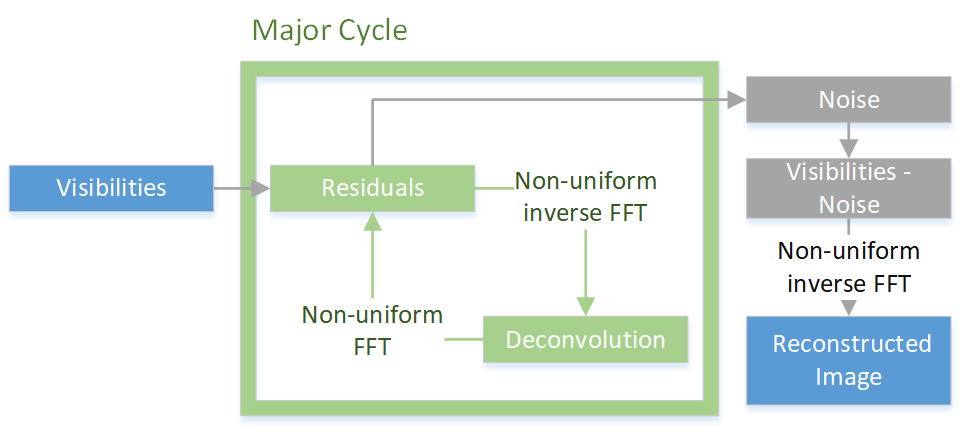
\includegraphics[width=1.0\linewidth]{./chapters/01.intro/Major-Minor.png}
	\caption{The Major Cycle Framework}
	\label{intro:major}
	\vspace{-10pt}
\end{wrapfigure}

The non-uniform FFT is responsible for approximating a regularly spaced image from the measurements, and for approximating the measurements corresponding to an image. Non-uniform FFT's are fast approximation algorithms, but by being approximation algorithms, they introduce errors. 

A optimization algorithm uses the image and removes the effect of incomplete samples. In the past, CLEAN algorithms were used to remove the effects. For the future, algorithms based on the theory of compressed sensing show promises in image quality.

A full major cycle consists of the following operations: First, it approximates the regularly spaced the regularly spaced image from the measurements. Then the optimization algorithm removes the effects of Incomplete measurements and returns the corresponding image. The major cycle then approximates the measurements corresponding to the image with the non-uniform FFT. The residual measurements are used in the next Major Cycle. In each cycle, two errors get simultaneously reduced:

\begin{enumerate}
	\item The Error introduced by the non-uniform FFT.
	\item The Error introduced by the incomplete measurements.
\end{enumerate}

After several major cycles the algorithm converges on a regularly spaced image which has a small error from non-uniform samples, and a small error from incomplete measurements.

For the optimization algorithm, the CLEAN class of algorithms get used. But algorithms based on the theory of compressed sensing have been shown to produce superior images.


\subsection{Compressed Sensing Reconstructions}
 However, compressed Sensing algorithms come with the drawback of requiring more major cycles.

MeerKAT due to wide field of view introduces even more troubles

Current Compressed Sensing reconstructions reduce the number of major cycles. However, the question is if Compressed Sensing can use a different architecture, and scale better to problems of the size of MeerKAT.

Furthermore on the new MeerKAT instruments, we have a big data problem. We want to create a large image from a large amount of Visibilities. 32k*32k pixels and terabytes of raw Visibility data. 

Scalability is a big problem.

There are ways to get rid of the major cycle, but overall the complexity could not be reduced.









